\documentclass{article}
\usepackage[utf8]{inputenc}
\usepackage{amsmath}
\usepackage{amssymb}
\usepackage{amsthm}
\usepackage{cancel}
\usepackage[shortlabels]{enumitem}
\usepackage{caption}
\usepackage{graphicx}
\usepackage[top=0.5in, bottom=0.5in, left=1in, right=1in]{geometry}
\usepackage{float}

% \usepackage{titlesec}
%     \titlespacing{\subsection}{\parindent}{15pt}{12pt}

\title{\textbf{\underline{CSCI4150U: Data Mining}\\Lab 02}}
\author{Syed Naqvi\\100590852}
\date{\today}

\begin{document}

    \maketitle
    
    \section*{Part I:}

    \subsection*{3.}
    
    \begin{center}
        \begin{minipage}[t]{0.9\textwidth}
            Since the class variable is a discrete feature, we can observe its
            distribution using a bar plot:
            \begin{figure}[H]
                \centering
                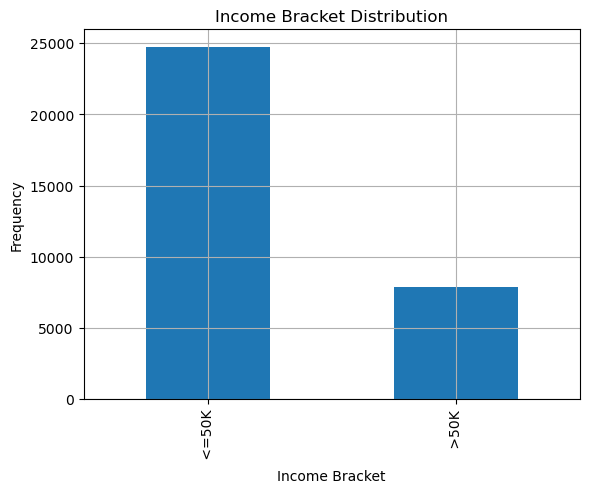
\includegraphics[width=0.8\textwidth, height=0.4\textheight]{./1_3.png}
            \end{figure}
            The diagram clearly shows that the majority of surveyed people (approximately 250000)
            earn less than or equal to 50k per year. This is roughly 3 times as many people
            (approximately 75000) who earn more than 50k per year.        
        \end{minipage}
    \end{center}

    \subsection*{4.}
    
    \begin{center}
        \begin{minipage}[t]{0.9\textwidth}
            Let us visualize the distributions of population age, education level and hours worked per week:
            \begin{figure}[H]
                \centering
                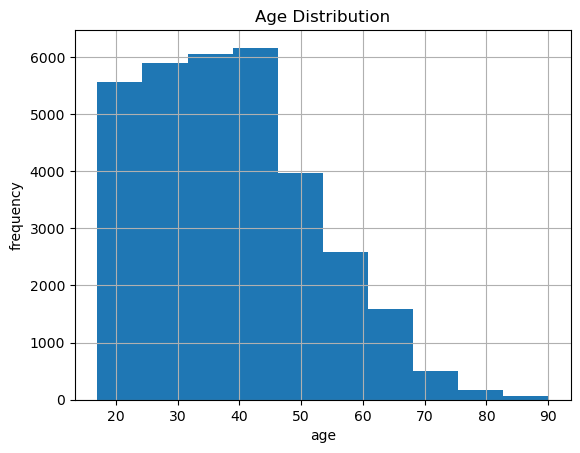
\includegraphics[width=0.8\textwidth, height=0.3\textheight]{./1_4a.png}
            \end{figure}
            From the age distribution we can see that the population mainly consists of more
            youthful individuals, with the overwhelming majority of people less than 50 years old.
            A younger demographic likely explains much of the over-representation of lower
            income individuals since income usually increases with age.
            \begin{figure}[H]
                \centering
                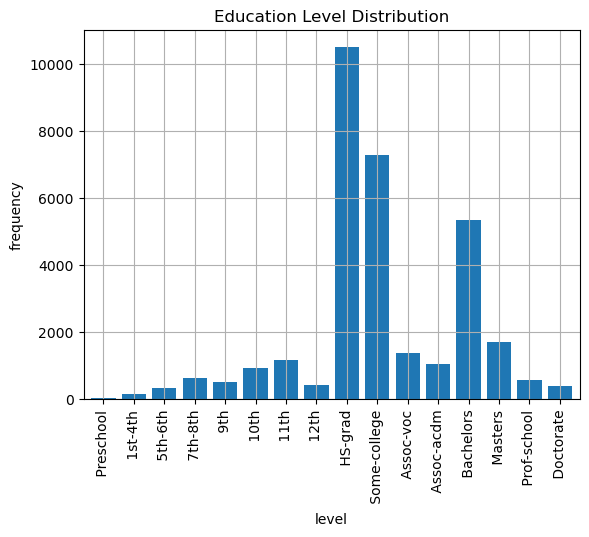
\includegraphics[width=0.8\textwidth, height=0.4\textheight]{./1_4b.png}
            \end{figure}
            The most common levels of educational attainment seem to be high school graduates,
            then some amount of college followed by bachelors degrees. The majority of people
            having less than a bachelors degree of education while also being relatively young
            further explains the higher degree of low income earners. 
        \end{minipage}
    \end{center}
    \newpage
    \begin{center}
        \begin{minipage}[t]{0.9\textwidth}
            \begin{figure}[H]
                \centering
                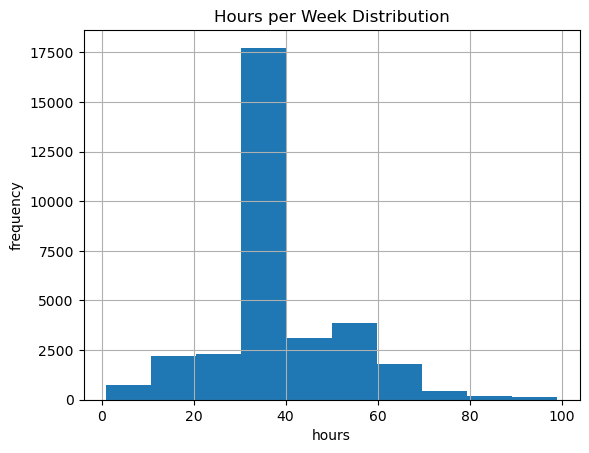
\includegraphics[width=0.8\textwidth, height=0.4\textheight]{./1_4c.png}
            \end{figure}
            The overwhelming majority of people seem to be working less than or
            equal to 40 hours per week. This indicates a higher likelihood of 9-5
            employees in the surveyed population as opposed to self-employed
            people or entrepreneurs who often work longer hours with higher earnings. 
        \end{minipage}
    \end{center}
    
    \subsection*{5.}
    
    \begin{center}
        \begin{minipage}[t]{0.9\textwidth}
            The following plot explores potential relationships between age and hours worked:
            \begin{figure}[H]
                \centering
                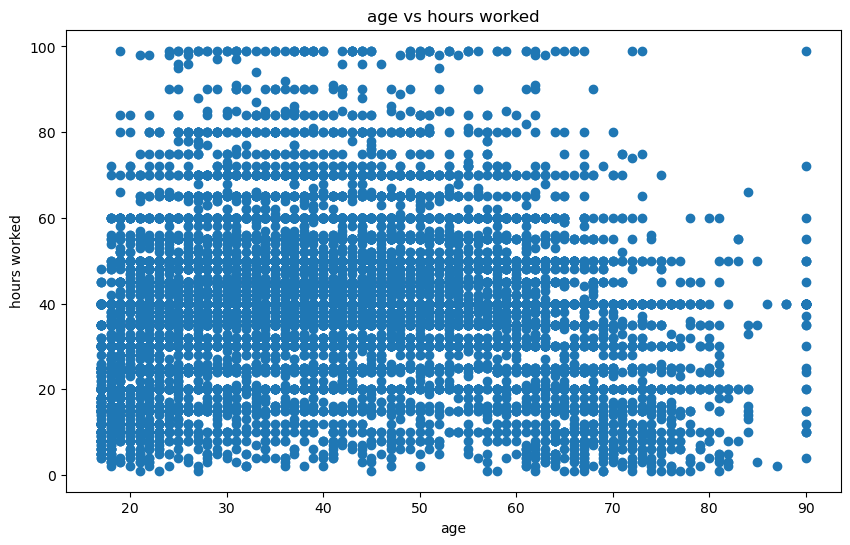
\includegraphics[width=0.8\textwidth, height=0.3\textheight]{./1_5a.png}
            \end{figure}
            While I had expected to see a stronger negative correlation where people
            work fewer hours as they age, there does seem to be some alighnemt with
            that notion in the way of a parabolic relationship.
            We can see that the majority of people in their late teens and early twenties
            start working with great variability in their number of hours. I imagine
            this is likely due to a mixture of part-time students and full-time entry
            level workers. The variability in the number of hours certainly appears to
            stabilize around 45 hours per week throughout middle age from late twenties
            to about 60. At this point people likely begin to retire or greatly reduce
            their workloads resulting in a more downward trend.
        \end{minipage}
    \end{center}

    \newpage

    \begin{center}
        \begin{minipage}[t]{0.9\textwidth}
            \begin{figure}[H]
                \centering
                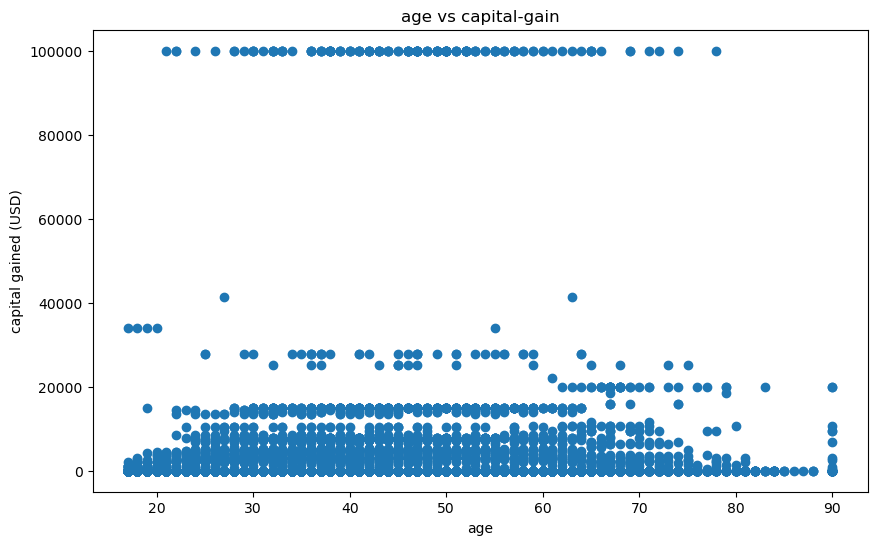
\includegraphics[width=0.8\textwidth, height=0.3\textheight]{./1_5b.png}
            \end{figure}
            \begin{figure}[H]
                \centering
                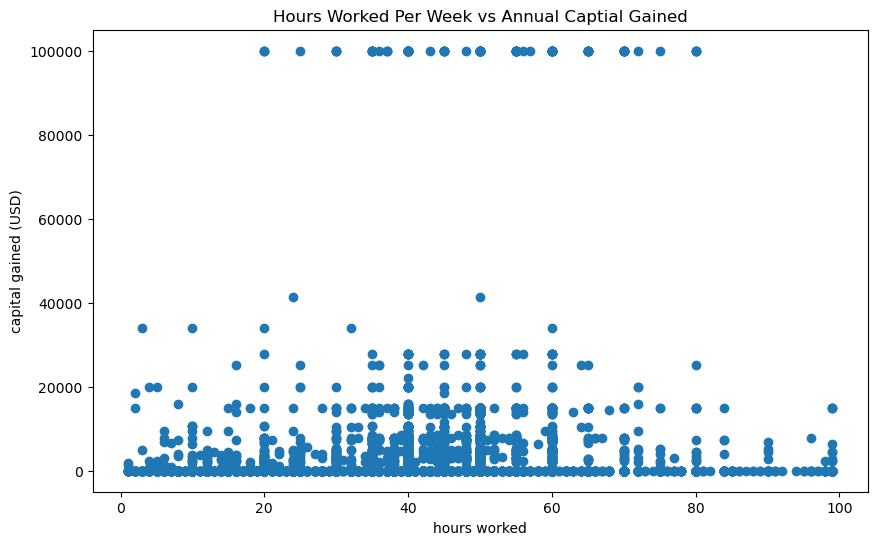
\includegraphics[width=0.8\textwidth, height=0.3\textheight]{./1_5c.png}
            \end{figure}
            Exploring the relationship between age vs captial gain as well as hours worked
            vs captial gain, we see very simlar distributions.
            It appears that the captial gains remains relatively stable throughout people's
            adult lives with a slight parabolic curve suggesting the majority of gains come
            around the 3rd quarter of life. It may be the case that with age come more
            accumulated assets that can be sold as well as better business sense.
            The hours worked vs captial gains plot appears very similar in shape where the
            majority of captial gains are made be people working roughly 50 hours per week.
            Perhaps working fewer hours than this means people are not generally wealthy enough
            to afford assets to sell and beyond this level of work there is not much
            time to invest in other affairs besides work.
            There does seem to be a set of outliers in the plots involving capital gains where
            a small subset earns nearly 100000 USD per year.
        \end{minipage}
    \end{center}

    \newpage

    \subsection*{6.}

    \begin{center}
        \begin{minipage}[t]{0.9\textwidth}
            \begin{figure}[H]
                \centering
                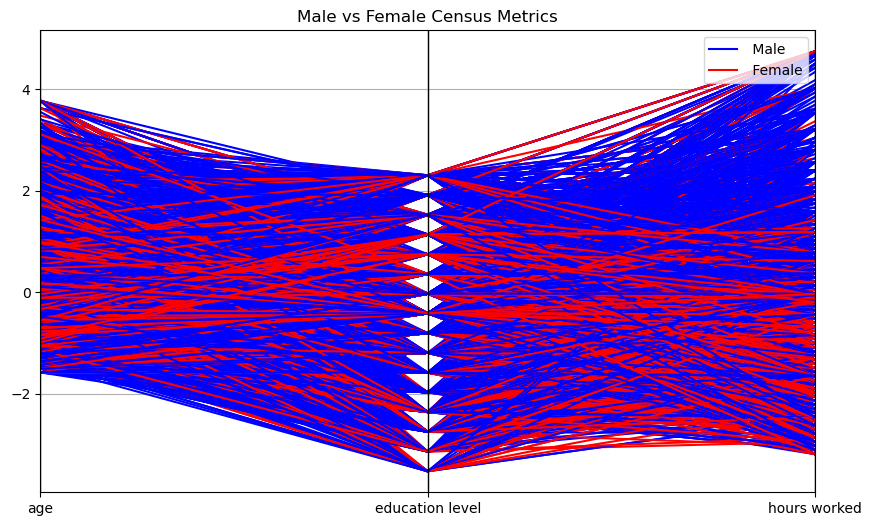
\includegraphics[width=1\textwidth, height=0.4\textheight]{./1_6a.png}
            \end{figure}
            The above figure contains standardized age, education level and hours worked axes
            in order to make the parallel graph more readable and patterns more apparent.
            We can see that males and females are genearlly represented equally across all metrics
            other than hours worked where we can clearly see that males are over-represented
            among the people with the most hours worked. There also seems to be a greater
            proportion of men among the upper and lower levels of education while women occupy
            more of the middle levels. I suspect the number of hours worked likely contributes
            to a subsequent gender pay gap. 
        \end{minipage}
    \end{center}

    \newpage

    \section*{Part II:}

    \subsection*{3.}

    \begin{center}
        \begin{minipage}[t]{0.9\textwidth}
            \begin{figure}[H]
                \centering
                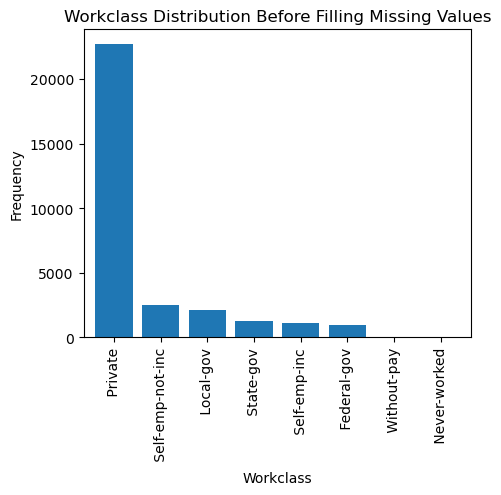
\includegraphics[width=0.8\textwidth, height=0.35\textheight]{./2_3ai.png}
            \end{figure}
            \begin{figure}[H]
                \centering
                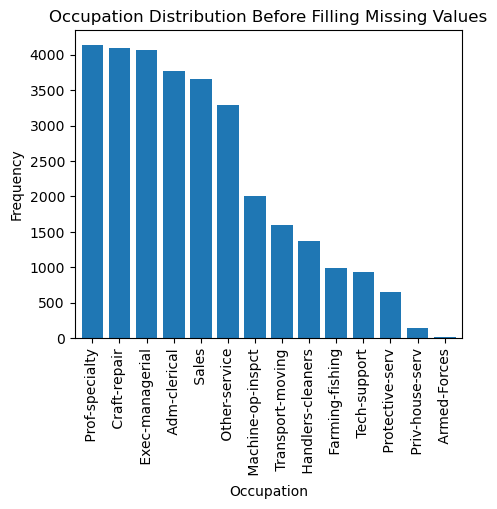
\includegraphics[width=0.8\textwidth, height=0.35\textheight]{./2_3aii.png}
            \end{figure}
        \end{minipage}
    \end{center}
    \newpage
    \begin{center}
        \begin{minipage}[t]{0.9\textwidth}
            \begin{figure}[H]
                \centering
                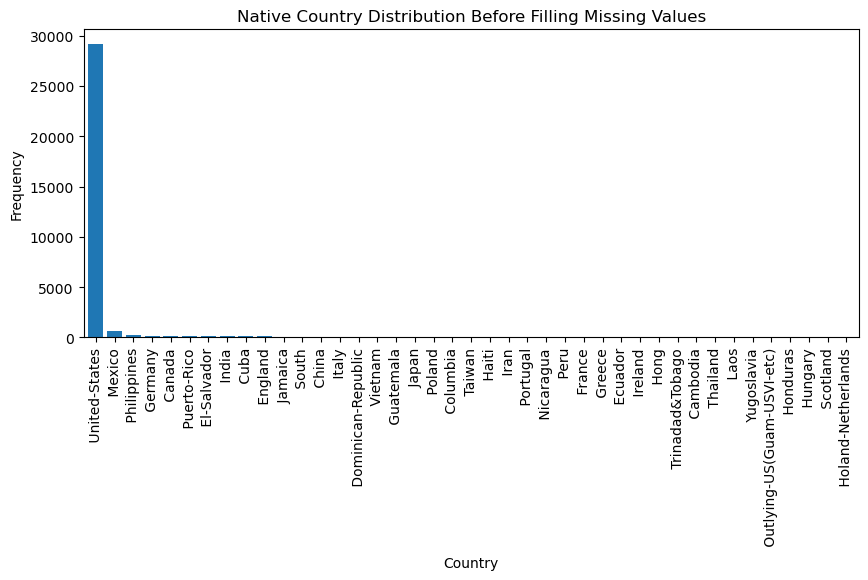
\includegraphics[width=1\textwidth, height=0.4\textheight]{./2_3aiii.png}
            \end{figure}
            The above three graphics visualize the distributions of the three
            features with NaN entires. Each feature was discrete and so its distribution was
            visualized using a bar gprah.
            For the above plots, records with missing entries were simply ignored.
        \end{minipage}
    \end{center}

    \begin{center}
        \begin{minipage}[t]{0.9\textwidth}
            \begin{figure}[H]
                \centering
                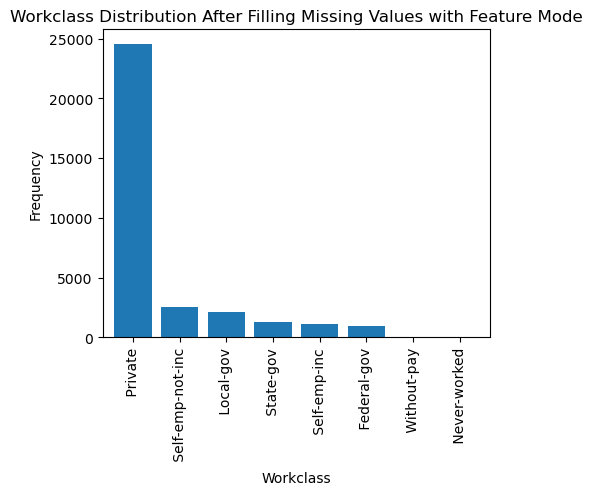
\includegraphics[width=1\textwidth, height=0.4\textheight]{./2_3bi.png}
            \end{figure}
        \end{minipage}
    \end{center}

    \newpage

    \begin{center}
        \begin{minipage}[t]{0.9\textwidth}
            \begin{figure}[H]
                \centering
                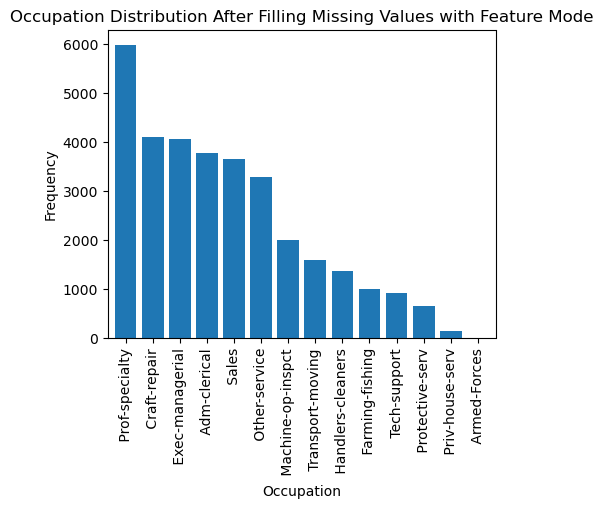
\includegraphics[width=1\textwidth, height=0.4\textheight]{./2_3bii.png}
            \end{figure}
            \begin{figure}[H]
                \centering
                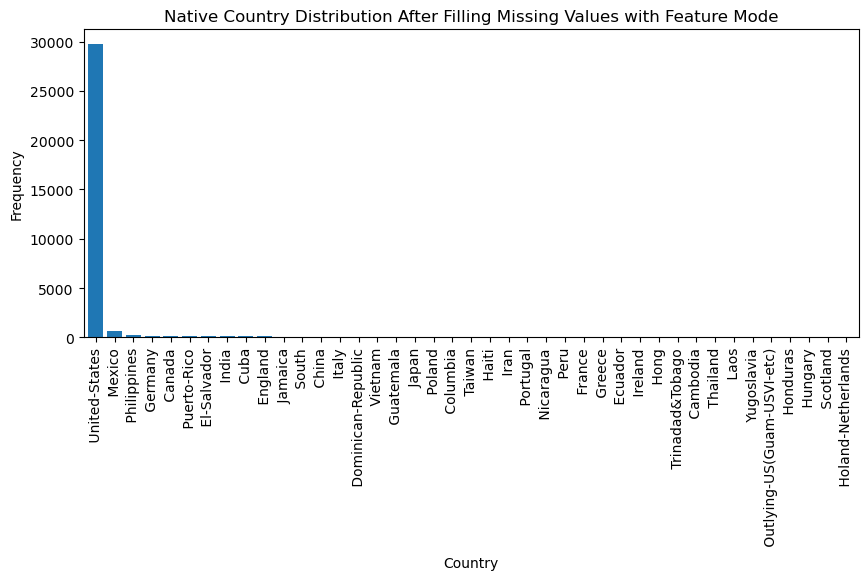
\includegraphics[width=1\textwidth, height=0.4\textheight]{./2_3biii.png}
            \end{figure}
            The above three graphics were generated after replacing NaN entries with the mode
            of their column. The effects of this are clearly reflected in the diagrams where
            the most frequent value in each distribution experienced a significant increase
            since all missing entries were set equal to this value.
            In the case of prof-specialty occupation, this value jumped from near 4000 to near
            6000.
        \end{minipage}
    \end{center}

    \newpage

    \begin{center}
        \begin{minipage}[t]{0.9\textwidth}
            \begin{figure}[H]
                \centering
                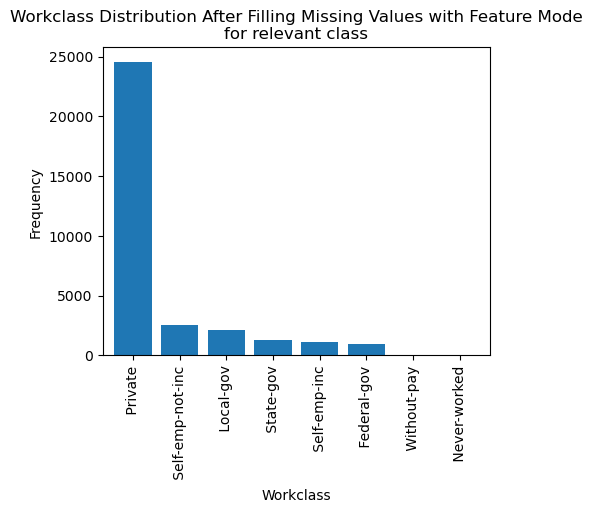
\includegraphics[width=1\textwidth, height=0.4\textheight]{./2_3ci.png}
            \end{figure}
            \begin{figure}[H]
                \centering
                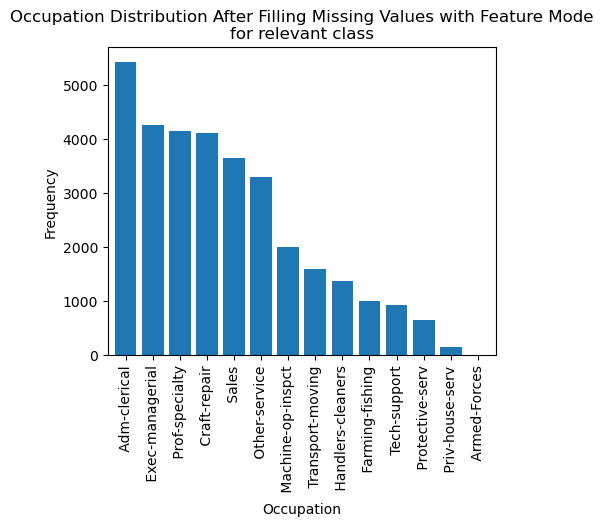
\includegraphics[width=1\textwidth, height=0.4\textheight]{./2_3cii.png}
            \end{figure}
        \end{minipage}
    \end{center}
    \begin{center}
        \begin{minipage}[t]{0.9\textwidth}
            \begin{figure}[H]
                \centering
                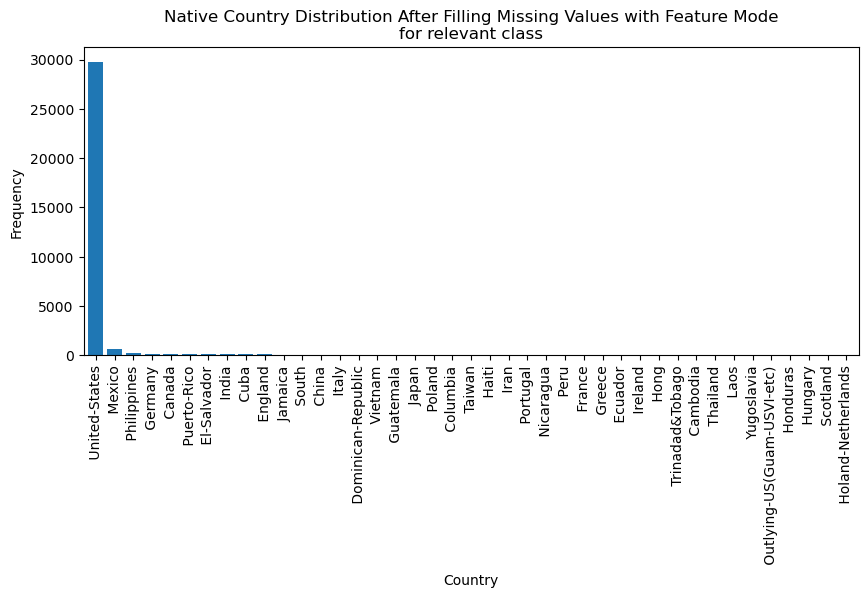
\includegraphics[width=1\textwidth, height=0.4\textheight]{./2_3ciii.png}
            \end{figure}
            We now see a slight decrease in some of the most frequent values since they
            are no longer necessarily the most frequent for their feature depending
            on the class of the instance. The missing values are thus being distributed
            among the top most frequent values, although the change is not too significant.
        \end{minipage}
    \end{center}


\end{document}